\documentclass[../../main.tex]{subfiles}

\graphicspath{{\subfix{../../immagini/}}}

\begin{document}
    Formalmente posso definire l'obiettivo dell'apprendimento supervisionato come:
    
    \begin{dfn}
        Dato un \textbf{training set} nella forma:
        \[(x_1, y_1), (x_2, y_2), \dots, (x_N, y_N)\]
        con ogni $y_i$ generato da una funzione ignota $y = f(x)$ trovare una funzione $h$, detta funzione \textbf{d'ipotesi}, o modello, che approssimi in modo accettabile la vera funzione $f$.
    \end{dfn}

    L'obiettivo è quindi ricercare nello spazio di tutte le possibili funzioni d'ipotesi una che approssimi la funzione $f$, \textit{anche su nuovi esempi non appartenenti al training set}, si dice in questo caso che $h$ è in grado di \textbf{generalizzare}.

    Esistono diverse \textbf{classi di funzione d'ipotesi}:
    \begin{itemize}
        \item Funzioni lineari
        \item Funzioni polinomiali grado N
        \item Funzioni sinusoidali
        \item Funzioni esponenziali
    \end{itemize}

    A prescindere dal tipo di classe utilizzata avrò una serie di \textbf{parametri}, ad esempio nel caso di una funzione lineare avrei:
    \[h(x) = w_0 + w_1x_1 + \dots + w_nx_n\]
    L'obiettivo è quindi \textit{fittare} la funzione d'ipotesi sui dati: trovare l'insieme di parametri che allineano il più possibile la funzione $h$ con i dati presenti nel training set. 

    A seconda di come la funzione $f$ è definita esistono due principali tipi di apprendimento supervisionato: nel caso in cui $f$ abbia come codominio $\mathbb{R}$ sono in un problema di \textbf{regressione}, se invece $f$ ha un codominio con un numero discreto e finito di elementi (Quindi assegna un'\textit{etichetta} ad ogni elemento dell'insieme di training) allora parlo di problema di \textbf{classificazione}.

    Prendendo come riferimento una funzione $h$ lineare vado ora ad analizzare i due casi di regressione e classificazione:

    \textbf{Regressione}: Partendo quindi da una funzione d'ipotesi definita come:
    \[h(x) = w_0 + w_1x_1 + w_2x_2 + \dots + w_nx_n = \bm{w^T x}\]
    Il problema in questo caso viene detto di \textbf{regressione lineare multi-variata}; l'idea è quella di sfruttare gli elementi dell'insieme di training a disposizione per trovare un vettore dei parametri $\bm{w}$ che permetta di minimizzare, per ognuno degli $y_i$, una funzione, chiamata di \textit{loss}, definita come la differenza tra $y_i$ e $h(x_i)$, solitamente viene utilizzata una funzione di loss quadratica:
    \[L(w) = \sum_{j=1}^N(y_j - h(x_j))^2\]
    Per minimizzare la funzione è necessario trovare dei parametri tali per cui la derivata di $L$, in funzione di tali parametri, sia pari a 0:
    \[\frac{\sigma}{\sigma w} L(h) = 0\]
    Nel caso della regressione lineare l'approccio più semplice è di risolvere analiticamente la derivata al fine di ricavare una funzione generale con cui calcolare direttamente il valore di ognuno dei parametri, prendendo il caso più semplice in cui $h$ è in una sola variabile ottengo le seguenti derivate:
    \[
    \begin{cases}
        w_0 = & \frac{\sum_{i=1}^N z_i - w_1 \sum_{i=1}^N}{N}\\
        w_1 = & \frac{N(\sum_{i=1}^N z_ix_i) - \sum_{i=1}^N z_i \sum_{i=1}^N x_i}{N(\sum_{i=1}^N x_i^2 - (\sum_{i=1}^N x_i)^2)} 
    \end{cases}    
    \]
    Non sempre però un approccio di questo tipo è possibile: non sempre infatti esiste una soluzione in forma chiusa della funzione $L$, in casi di questo tipo solitamente si ricorre ad un approccio \textit{iterativo} più generale (https://stats.stackexchange.com/questions/23128/solving-for-regression-parameters-in-closed-form-vs-gradient-descent) con algoritmi che sfruttano il gradiente della funzione $L$, nel nostro caso utilizzeremo un algoritmo di \textbf{discesa del gradiente}, in quanto l'obiettivo è di \textit{minimizzare} il valore della perdita.

    Intuitivamente l'algoritmo lavora non più sulla perdita calcolata su tutto il dataset ma analizzando gli elementi di tale insieme uno alla volta ed aggiornando il valore dei pesi di conseguenza, sottoforma di pseudocodice l'algoritmo ha la seguente forma:

    $\bf{w} \leftarrow \text{Punto d'inizializzazione}$\\
    \textbf{do}:\\
    - \quad \textbf{foreach $w_i$ in $\bf{w}$}:\\
    - \quad \quad $w_i \leftarrow w_i - \alpha \frac{\sigma}{\sigma w_i} L(\bf{w})$\\
    \textbf{while} (not convergenza)

    Dove $\alpha$, chiamato \textbf{learning rate}, rappresenta la "forza" della modifica dei pesi ad ogni passo.

    Utilizzando ancora una volta una perdita quadratica (Questa volta però calcolata sui singoli elementi dell'insieme di addestramento):
    \[L(\bf{w}) = \frac{1}{2}(y_j - h(\bf{x_j}))^2\]
    L'aggiornameto dei pesi ad ogni passo verrebbe calcolato come:
    \[\frac{\sigma L(\bf{w})}{\sigma w_i} = \frac{1}{2}\frac{\sigma(y_j - h(\bf{x_j}))^2}{\sigma w_i} = - (y_j - h(\bf{x_j})) x_i\]
    \[w_i \leftarrow w_i + \alpha (z_j - h(\bf{x_j})) x_i\]
    \begin{figure}[h!]
        \centering
        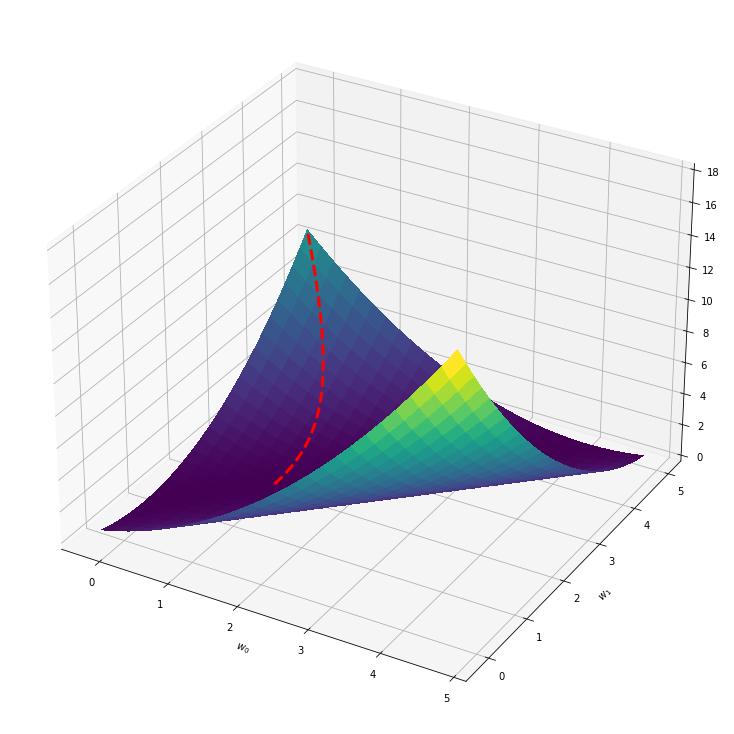
\includegraphics[width = \textwidth/2]{immagini/4_1/loss_function.png}
        \caption{Esempio del funzionamento dell'algoritmo del gradiente utilizzato per aggiornare il valore dei pesi: noto come il valore della funzione di perdita diminuisca all'aumentare del numero di iterazioni fino ad arrivare a convergenza}
    \end{figure}
   

    \textbf{Classificazione}: Se la funzione $f$ da approssimare ha un codominio discreto si parla di classificazione, in questo contesto i metodi per la regressione possono essere riadattati per affrontare questa tipologia di problemi: il modello calcola un punteggio a cui si applica una soglia.

    Un modello lineare può ad esempio essere utilizzato anche nel contesto dei problemi di classificazione: ad esempio in figura si può vedere un insieme di punti appartenenti a due classi differenti, in generale si definisce \textbf{decision boundary} la linea che separa i punti delle due classi, se tale boundary è, come nell'esempio, una linea retta si parla di classi \textit{linearmente separabili}. Per adattare questo approccio al caso della classificazione semplicemente definisco una \textit{soglia}: se un determinato elemento assume un valore $> 0$ nella funzione $h$ allora $h(x) = 1$ altrimenti $h(x) = 0$, formalmente posso quindi pensare di far passare il risultato di $h$ in una funzione di soglia ed utilizzare tale risultato come classe risultante:
    \[h\bf(x) = Soglia(\bf{w} \cdot \bf{x}) \ \text{con} \ Soglia(z) = 1 \ \text{se} \ z \geq 0 \ \text{altrimenti} \ 0\]
    Noto come defininendo in questo modo il modello sia non sia però possibile aggiornare i pesi utilizzando lo stesso approccio adottato nel caso della regressione: il gradiente di $h$ è infatti sempre pari a 0 tranne nei punti in cui $\bf{w} \cdot \bf{x} = 0$ in cui però è indefinito.
    
    La soluzione è quella di utilizzare la \textbf{percepron learning rule}:
    \[w_i \leftarrow w_i + \alpha (y - h(\bf{x})) x_i\]
    lavorando su problemi di classificazione binaria 0/1 questa regola intuitivamente aggiornerà i pesi solamente nel caso in cui il risultato del modello sia errato.

\end{document}